%%%%%%%%%%%%%%%%%%%%%%%%%%%%%%%%%%%%%%%%%%%%%%%%%%%%%%%%%%%%%%%%%%%%%%%%
%% Customizações do abnTeX2 (http://abnTeX2.googlecode.com)           %%
%% para a Universidade Estadual do Ceara - UECE                       %%
%%                                                                    %%
%% This work may be distributed and/or modified under the             %% 
%% conditions of the LaTeX Project Public License, either version 1.3 %%
%% of this license or (at your option) any later version.             %%
%% The latest version of this license is in                           %%
%%   http://www.latex-project.org/lppl.txt                            %%
%% and version 1.3 or later is part of all distributions of LaTeX     %%
%% version 2005/12/01 or later.                                       %%
%%                                                                    %%
%% This work has the LPPL maintenance status `maintained'.            %%
%%                                                                    %%
%% The Current Maintainer of this work is Thiago Nascimento           %%
%%                                                                    %%
%% Project available on: https://github.com/thiagodnf/uecetex2        %%
%%                                                                    %%
%% Further information about abnTeX2                                  %%
%% are available on http://abntex2.googlecode.com/                    %%
%%                                                                    %%
%%%%%%%%%%%%%%%%%%%%%%%%%%%%%%%%%%%%%%%%%%%%%%%%%%%%%%%%%%%%%%%%%%%%%%%%

%%%%%%%%%%%%%%%%%%%%%%%%%%%%%%%%%%%%%%%%%%%%%%%%%%%%%%%%%%%%%%%%%%%%%%%%
%% Customizações do abnTeX2 (http://abnTeX2.googlecode.com)           %%
%% para a Universidade Estadual do Ceara - UECE                       %%
%%                                                                    %%
%% This work may be distributed and/or modified under the             %% 
%% conditions of the LaTeX Project Public License, either version 1.3 %%
%% of this license or (at your option) any later version.             %%
%% The latest version of this license is in                           %%
%%   http://www.latex-project.org/lppl.txt                            %%
%% and version 1.3 or later is part of all distributions of LaTeX     %%
%% version 2005/12/01 or later.                                       %%
%%                                                                    %%
%% This work has the LPPL maintenance status `maintained'.            %%
%%                                                                    %%
%% The Current Maintainer of this work is Thiago Nascimento           %%
%%                                                                    %%
%% Project available on: https://github.com/thiagodnf/uecetex2        %%
%%                                                                    %%
%% Further information about abnTeX2                                  %%
%% are available on http://abntex2.googlecode.com/                    %%
%%                                                                    %%
%%%%%%%%%%%%%%%%%%%%%%%%%%%%%%%%%%%%%%%%%%%%%%%%%%%%%%%%%%%%%%%%%%%%%%%%

\documentclass[        
    a4paper,          % Tamanho da folha A4
    12pt,             % Tamanho da fonte 12pt
    chapter=TITLE,    % Todos os capitulos devem ter caixa alta
    section=TITLE,    % Todas as secoes devem ter caixa alta
    oneside,          % Usada para impressao em apenas uma face do papel
    english,          % Hifenizacoes em ingles
    spanish,          % Hifenizacoes em espanhol
    brazil            % Ultimo idioma eh o idioma padrao do documento
]{abntex2}

% Importações de pacotes
\usepackage[utf8]{inputenc}                         % Acentuação direta
\usepackage[T1]{fontenc}                            % Codificação da fonte em 8 bits
\usepackage{graphicx}                               % Inserir figuras
\usepackage{amsfonts, amssymb, amsmath}             % Fonte e símbolos matemáticos
\usepackage{booktabs}                               % Comandos para tabelas
\usepackage{verbatim}                               % Texto é interpretado como escrito no documento
\usepackage{multirow, array}                        % Múltiplas linhas e colunas em tabelas
\usepackage{indentfirst}                            % Endenta o primeiro parágrafo de cada seção.
\usepackage{listings}                               % Utilizar codigo fonte no documento
\usepackage{xcolor}
\usepackage{microtype}                              % Para melhorias de justificação?
\usepackage[portuguese,ruled,lined]{algorithm2e}    % Escrever algoritmos
\usepackage{algorithmic}                            % Criar Algoritmos  
%\usepackage{float}                                  % Utilizado para criação de floats
\usepackage{amsgen}
\usepackage{lipsum}                                 % Usar a simulação de texto Lorem Ipsum
%\usepackage{titlesec}                               % Permite alterar os títulos do documento
\usepackage{tocloft}                                % Permite alterar a formatação do Sumário
\usepackage{etoolbox}                               % Usado para alterar a fonte da Section no Sumário
\usepackage[nogroupskip,nonumberlist,acronym]{glossaries}                % Permite fazer o glossario
\usepackage{caption}                                % Altera o comportamento da tag caption
\usepackage[alf, abnt-emphasize=bf, bibjustif, recuo=0cm, abnt-etal-cite=3, abnt-etal-list=0,abnt-etal-text=it]{abntex2cite}  % Citações padrão ABNT
%\usepackage[bottom]{footmisc}                      % Mantém as notas de rodapé sempre na mesma posição
%\usepackage{times}                                 % Usa a fonte Times
\usepackage{mathptmx}                               % Usa a fonte Times New Roman										
%\usepackage{lmodern}                               % Usa a fonte Latin Modern
%\usepackage{subfig}                                % Posicionamento de figuras
%\usepackage{scalefnt}                              % Permite redimensionar tamanho da fonte
%\usepackage{color, colortbl}                       % Comandos de cores
%\usepackage{lscape}                                % Permite páginas em modo "paisagem"
%\usepackage{ae, aecompl}                           % Fontes de alta qualidade
%\usepackage{picinpar}                              % Dispor imagens em parágrafos
%\usepackage{latexsym}                              % Símbolos matemáticos
%\usepackage{upgreek}                               % Fonte letras gregas
\usepackage{appendix}                               % Gerar o apendice no final do documento
\usepackage{paracol}                                % Criar paragrafos sem identacao
\usepackage{lib/uecetex2}		                    % Biblioteca com as normas da UECE para trabalhos academicos
\usepackage{pdfpages}                               % Incluir pdf no documento
\usepackage{amsmath}                                % Usar equacoes matematicas
%\usepackage{url}
\usepackage{hyperref}
\usepackage{textcomp}

% Organiza e gera a lista de abreviaturas, simbolos e glossario
\makeglossaries

% Gera o Indice do documento
\makeindex

\lstset{basicstyle=\ttfamily,
	showstringspaces=false,
	commentstyle=\color{red},
	keywordstyle=\color{blue}
}

\lstdefinestyle{BashInputStyle}{
  language=bash,
  basicstyle=\small\sffamily,
  numbers=left,
  numberstyle=\tiny,
  numbersep=3pt,
  frame=tb,
  columns=fullflexible,
  backgroundcolor=\color{yellow!20},
  linewidth=0.9\linewidth,
  xleftmargin=0.1\linewidth
}


%%%%%%%%%%%%%%%%%%%%%%%%%%%%%%%%%%%%%%%%%%%%%%%%%%%%%
%%          Configuracoes do ueceTeX2              %%
%%%%%%%%%%%%%%%%%%%%%%%%%%%%%%%%%%%%%%%%%%%%%%%%%%%%%

% Opcoes disponiveis

\trabalhoacademico{tccgraduacao}
%\trabalhoacademico{tccespecializacao}
%\trabalhoacademico{dissertacao}
%\trabalhoacademico{tese}

% Define se o trabalho eh uma qualificacao
% Coloque 'nao' para versao final do trabalho

\ehqualificacao{nao}

% Remove as bordas vermelhas e verdes do PDF gerado
% Coloque 'sim' pare remover

\removerbordasdohyperlink{sim} 

% Adiciona a cor Azul a todos os hyperlinks

\cordohyperlink{nao}

%%%%%%%%%%%%%%%%%%%%%%%%%%%%%%%%%%%%%%%%%%%%%%%%%%%%%
%%          Informação sobre a IES                 %%
%%%%%%%%%%%%%%%%%%%%%%%%%%%%%%%%%%%%%%%%%%%%%%%%%%%%%

\ies{FUNDAÇÃO CENTRO DE ANÁLISE, PESQUISA E INOVAÇÃO TECNOLÓGICA.}
\iessigla{CESF}
\centro{Instituto de Ensino Superior FUCAPI}

%%%%%%%%%%%%%%%%%%%%%%%%%%%%%%%%%%%%%%%%%%%%%%%%%%%%%
%%        Informação para TCC de Graduacao         %%
%%%%%%%%%%%%%%%%%%%%%%%%%%%%%%%%%%%%%%%%%%%%%%%%%%%%%

\graduacaoem{Sistemas de Informação}
\habilitacao{Bacharel} % Pode colocar tambem 'licenciada'
\areadeconcentracaograduacao{Ciência da Computação}

%%%%%%%%%%%%%%%%%%%%%%%%%%%%%%%%%%%%%%%%%%%%%%%%%%%%%
%%     Informação para TCC de Especializacao       %%
%%%%%%%%%%%%%%%%%%%%%%%%%%%%%%%%%%%%%%%%%%%%%%%%%%%%%

\especializacaoem{Alfabetização de Crianças}

%%%%%%%%%%%%%%%%%%%%%%%%%%%%%%%%%%%%%%%%%%%%%%%%%%%%%
%%         Informação para Dissertacao             %%
%%%%%%%%%%%%%%%%%%%%%%%%%%%%%%%%%%%%%%%%%%%%%%%%%%%%%

\programamestrado{Programa de Pós-Graduação em Ciência da Computação}
\nomedomestrado{Mestrado Acadêmico em Ciência da Computação}
\mestreem{Ciência da Computação}
\areadeconcentracaomestrado{Ciência da Computação}

%%%%%%%%%%%%%%%%%%%%%%%%%%%%%%%%%%%%%%%%%%%%%%%%%%%%%
%%               Informação para Tese              %%
%%%%%%%%%%%%%%%%%%%%%%%%%%%%%%%%%%%%%%%%%%%%%%%%%%%%%

\programadoutorado{Programa de Pós-Graduação em Saúde Coletiva}
\nomedodoutorado{Doutorado em Saúde Coletiva}
\doutorem{Saúde Coletiva}
\areadeconcentracaodoutorado{Saúde Coletiva}

%%%%%%%%%%%%%%%%%%%%%%%%%%%%%%%%%%%%%%%%%%%%%%
%%  Informação relacionadas ao trabalho     %%
%%%%%%%%%%%%%%%%%%%%%%%%%%%%%%%%%%%%%%%%%%%%%%

\autor{Marcelo Barbosa da Rocha}
\titulo{Protótipo de Sistema de Beacon baseado em rede Wifi}
\data{2015}
\local{Manaus}

% Exemplo: \dataaprovacao{01 de Janeiro de 2012}
\dataaprovacao{}

%%%%%%%%%%%%%%%%%%%%%%%%%%%%%%%%%%%%%%%%%%%%%
%%     Informação sobre o Orientador       %%
%%%%%%%%%%%%%%%%%%%%%%%%%%%%%%%%%%%%%%%%%%%%%

\orientador{Carlos Augusto de Araújo Mar}
\orientadorsiglatitulo{M.Sc.}
\orientadories{Universidade Estadual do Ceará – UECE}
\orientadorcentro{Centro de Ciências e Tecnologia - CCT}
\orientadorfeminino{nao} % Coloque 'sim' se for do sexo feminino

%%%%%%%%%%%%%%%%%%%%%%%%%%%%%%%%%%%%%%%%%%%%%
%%      Informação sobre o Co-orientador   %%
%%%%%%%%%%%%%%%%%%%%%%%%%%%%%%%%%%%%%%%%%%%%%

% Deixe o nome do coorientador em branco para remover do documento

\coorientador{}
\coorientadories{Universidade Co-orientador - SIGLA}
\coorientadorcentro{Centro do Co-orientador - SIGLA}
\coorientadorfeminino{nao} % Coloque 'sim' se for do sexo feminino

%%%%%%%%%%%%%%%%%%%%%%%%%%%%%%%%%%%%%%%%%%%%%
%%      Informação sobre a banca           %%
%%%%%%%%%%%%%%%%%%%%%%%%%%%%%%%%%%%%%%%%%%%%%

% Atenção! Deixe o nome do membro da banca para remover da folha de aprovacao

% Exemplo de uso:
% \membrodabancadois{Prof. Dr. Fulano de Tal}
% \membrodabancadoisies{Universidade Estadual do Ceará - UECE}

\membrodabancadois{Membro da Banca Dois}
\membrodabancadoiscentro{Faculdade de Filosofia Dom Aureliano Matos – FAFIDAM}
\membrodabancadoisies{Universidade do Membro da Banca Dois - SIGLA}
\membrodabancatres{Membro da Banca Três}
\membrodabancatrescentro{Centro de Ciências e Tecnologia - CCT}
\membrodabancatresies{Universidade do Membro da Banca Três - SIGLA}
\membrodabancaquatro{Membro da Banca Quatro}
\membrodabancaquatrocentro{Centro de Ciências e Tecnologia - CCT}
\membrodabancaquatroies{Universidade do Membro da Banca Quatro - SIGLA}
\membrodabancacinco{Membro da Banca Cinco}
\membrodabancacincocentro{Teste}
\membrodabancacincoies{Universidade do Membro da Banca Cinco - SIGLA}
\membrodabancaseis{Membro da Banca Seis}
\membrodabancaseiscentro{}
\membrodabancaseisies{Universidade do Membro da Banca Seis - SIGLA}

\begin{document}	

	% Elementos pré-textuais
	\imprimircapa
	\imprimirfolhaderosto{}
	\imprimirfichacatalografica{elementos-pre-textuais/ficha-catalografica}
	%\imprimirerrata{elementos-pre-textuais/errata}
	\imprimirfolhadeaprovacao
	\imprimirdedicatoria{elementos-pre-textuais/dedicatoria}
	%\imprimiragradecimentos{elementos-pre-textuais/agradecimentos}
	%\imprimirepigrafe{elementos-pre-textuais/epigrafe}
	%\imprimirresumo{elementos-pre-textuais/resumo}
	%\imprimirabstract{elementos-pre-textuais/abstract}
	%\imprimirlistadeilustracoes
	%\imprimirlistadetabelas
	%\imprimirlistadequadros
	%\imprimirlistadealgoritmos
	%\imprimirlistadecodigosfonte
	%\imprimirlistadeabreviaturasesiglas	
	%\imprimirlistadesimbolos{elementos-pre-textuais/lista-de-simbolos}   
	%\imprimirsumario
	
	%Elementos textuais
	\textual
	\chapter{Introdução}
\label{cap:introducao}

A internet das coisas segundo Ashton (2009) refere-se a convergência tecnológica onde as coisas do mundo real, ou seja, objetos usados no nosso dia-a-dia estarão conectados entre si e a rede de mundial de computadores. Nesse novo mundo as “coisas” conectadas passarão a ser mais inteligentes, coletar informações ao seu redor e realizar tarefas automaticamente sem a interferência humana. \\
\indent Em meio aos vários objetos que aos poucos estão dando forma a internet das coisas estão os beacons. Beacons são pequenos dispositivos que utilizam a tecnologia bluetooth para detectar a presença de outros dispositivos (smartphones, tablets, etc), dentro do seu raio, que também tenham bluetooth ativo e iniciar uma ação nesses mesmos dispositivos através de um aplicativo intermediário previamente instalado. \\
\indent Os beacons podem agir de forma ativa, permitindo que as aplicações com que eles interagem, possam prover aos usuários informações com base no seu contexto de localização. Ou de forma passiva simplesmente registrando que um determinado dispositivo entrou em seu raio de detecção, esses registros podem ser trabalhados por outros sistemas para obter a localização aproximada do usuário em relação ao beacon. \\
\indent A aplicabilidade dos beacons são diversas. Podem ser utilizados para mapeamento de fluxo de usuários em shoppings, feiras e eventos diversos; localização em ambientes fechados (indoor); ou em uma loja de varejo, enviar uma notificação com informação de ofertas de produtos para os smartphones de clientes quando eles passarem por uma determinada área da loja. Também existem outras possibilidades, como: checkins automáticos e até pagamentos através de dispositivos móveis.



\section{Problema}
\label{sec:problema}

Segundo Teixeira (2014) beacons não são inteligentes, toda a inteligência fica sob responsabilidade do aplicativo instalado no dispositivo que irá interagir com o beacon. Atualmente no mercado existem dois padrões principais para comunicação entre beacons e aplicações, o iBeacon criando e mantido pela Apple, é um padrão proprietário que funciona somente com os dispositivos da própria fabricante e o Eddystone criando e mantido pela Google, é um padrão aberto (open-source) que pode ser utilizado por qualquer dispositivo. Em ambos os padrões o beacon age conforme a afirmação anterior, a total dependência de uma aplicação pode representar um problema em alguns casos, como por exemplo no cenário em que uma loja de varejo deseja utilizar beacons para prover informações para os seus clientes com base nos dados de seus próprios perfis e também histórico das últimas compras realizadas, que estão armazenados em seus servidores de banco de dados, mas não deseja disponibilizar por razões de segurança, um serviço público que exponha os dados dos clientes diretamente para um aplicativo. \\
\indent Neste último cenário seria mais seguro que os dados podessem ser tratados, caso fosse necessário, pelo próprio beacon antes de serem enviados para a aplicação instalada no dispositivo do cliente que está interagindo com ele. Além disso, o acesso do serviço sendo realizado através do beacon representa mais segurança para a rede interna da loja, pois neste cenário o beacon é um dispositivo que pode ser controlado pelo próprio administrador da rede.

\section{Objetivos}
\label{sec:objetivos}

Neste tópico serão abordados os objetivos geral e específicos desta monografia.

\subsection{Objetivo Geral}
\label{sec:objetivo-geral}

Desenvolver um protótipo de sistema de beacon baseado na tecnologia wifi para aumentar a taxa de transferência de dados e a segurança de aplicações baseadas em beacons bluetooth.

\subsection{Objetivos Específicos}
\label{sec:objetivos-especificos}

	\begin{itemize}
		\item Pesquisar e definir as tecnologias, ferramentas e suas configurações para criar o beacon wifi;
		\item Implementar o algoritmo do protocolo de comunicação para o beacon e os dispositivos;
		\item Desenvolver o aplicativo cliente para comunicação;
		\item Desenvolver um serviço para prover as informações para o sistema utilizando o beacon e o aplicativo cliente;
		\item Validar o protótipo quanto ao aumento da taxa de transferência de dados e segurança.
	\end{itemize}

\section{Justificativa}
\label{sec:justificativa}

Seguindo o propósito da internet das coisas, em disponibilizar dispositivos cada vez mais inteligentes que possam executar tarefas automaticamente sem a intervenção humana, este trabalho tem o intuito de desenvolver um beacon capaz não somente de detectar a presença dos dispositivos que entrarem em seu raio de ação, mas também um beacon mais inteligente que os encontrados atualmente no mercado, podendo processar dados internamente e também comunicar diretamente com serviços internos ou externos.

\section{Trabalhos Relacionados}
\label{sec:trabalhos-relacionados}

Choi, Park e Lee (2015) descreveram um sistema de gerenciamento de energia de escritório capaz de reduzir o consumo de energia de computadores, monitores e luzes de um escritório com a utilização de beacons baseados em bluetooth e um aplicativo móvel. Enquanto vários beacons foram colocados em lugares estratégicos do escritório de forma a cobrir todos os espaços, um aplicativo móvel determina, com a ajuda dos beacons, se o usuário entrou ou saiu do escritório e modificam o modo de economia de energia dos computadores, monitores e luzes. O sistema proposto pode reduzir o consumo de energia em um escritório sem causar desconforto aos usuários. No caso da utilização de beacons wifi, com um único dispositivo, seria possível cobrir toda uma sala do escritório. \\
\indent Bohonos et al. (2007) descreveram um sistema de software e hardware chamado URNA (Universal Real-Time Navigational Assistance) que permite a comunicação de informações relevantes de localização para uma pessoa cega através de um celular com bluetooth. O sistema tem como alvo principal ajudar um pedestre cego na travessia de ruas de um cruzamento, informando o nome da rua e o estado atual do semáforo. Com o uso de beacon wifi, visto que a tecnologia bluetooth tem um curto alcance, o sistema poderia ser estendido com a criação de um aplicativo para os motoristas, cuja a funcionalidade seria comunicar com o beacon e informá-los sobre a presença de pedestres cegos a medida que o mesmo se aproximasse de um semáforo. \\
\indent Chawathe (2008) descreve um método de localização de dispositivos móveis em ambientes fechados usando beacons baseados em bluetooth. Nesse caso o raio de detecção limitado da tecnologia bluetooth é usado como vantagem. Mas para isso é preciso estabelecer de forma correta a posição de cada beacon, de modo que os beacons não sofram com interferência de raio de outro beacon.

\section{Método de Investigação}
\label{sec:metodo-investigacao}

A metodologia de desenvolvimento proposta para este trabalho é composta das seguintes etapas: \\
\indent A pesquisa de referencial teórico sobre beacons será baseada nas principais fontes encontradas no mercado e/ou disponibilizado na internet, como livros, artigos, tutoriais e revistas. Com intuito de fornecer ao trabalho um embasamento teórico necessário para o entendimento dos beacons, os conceitos envolvidos e suas características. \\
\indent A pesquisa de tecnologias e ferramentas necessárias para definição da arquitetura e construção de um beacon baseado na tecnologia wifi utilizando o microcomputador Raspberry Pi, juntamente com seu sistema operacional raspbian baseado na distribuição linux debian. Bem como a forma de detecção dos dispositivos cliente; e também o protocolo de comunicação a ser utilizado entre o beacon e esses dispositivos. \\
\indent Na etapa de desenvolvimento serão implementados: o protótipo do aplicativo cliente que fará uso das principais ferramentas encontradas para o desenvolvimento android, sendo o Android Studio como ambiente integrado de desenvolvimento (IDE) e o Framework Android; e o serviço responsável por implementar o protocolo de comunicação definido na etapa anterior. Como objetivo desta etapa, o aplicativo deverá ser capaz de entender e utilizar o serviço de protocolo de comunicação com o beacon para o recebimento de suas mensagens em forma de notificação. \\
\indent Na etapa de validação da solução ocorrerá a comparação dos resultados obtidos a respeito da capacidade máxima do raio de detecção dos dispositivos clientes, a rapidez na transferência dos dados aos dispositivos e o nível de segurança proporcionado na utilização da tecnologia wifi no beacon em relação a tecnologia bluetooth. \\
\indent A etapa de escrita a monografia acontecerá durante todo o período de execução deste trabalho.

\section{Estruturação da Monografia}
\label{sec:estruturacao-monografia}

XXXXXXXXXXXXXXXXXXXXXXXXX

\section{Cronograma}
\label{sec:cronograma}

XXXXXXXXXXXXXXXXXXXXXXXXX
	%\chapter{Fundamentação Teórica}
\label{cap:fundamentacao-teorica}

Este capítulo tem por finalidade apresentar os principais conceitos necessários para o desenvolvimento do presente trabalho. Serão abordados 

\section{Beacons}
\label{sec:beacons}

\cite{Danova} conceitua que beacons são dispositivos de hardware de baixo custo que são pequenos o suficiente para serem fixados em uma parede ou um balcão. Eles utilizam bateria de forma eficiente e conexão bluetooth low energy (de baixo consumo) para enviar mensagens ou notificações para smartphones ou tablets.

\begin{figure}[h!]
	\centering
	\Caption{\label{fig:exemplo-1} Beacons}	
	\UECEfig{}{
		\fbox{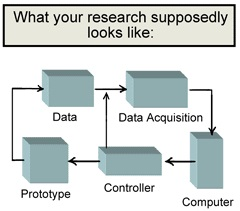
\includegraphics[width=8cm]{figuras/figura-1}}
	}{
	\Fonte{Estimote}			
}	
\end{figure}

\indent Os beacons são considerados dispositivos integrantes da próxima geração da internet, chamada de internet das coisas, onde terão um papel fundamental na forma de comunicação entre as mais variadas instituições como: lojas de varejo, locais de eventos, supermercados, restaurantes e instituições de ensino; e as pessoas. \\
\indent Entre os padrões de beacons existentes atualmente no mercado, dois se destacam por serem desenvolvidos pelas duas empresas -- Apple e Google -- mais importantes e inovadoras da área tecnológica. A seguir, os padrões serão explicados com detalhes. 


\subsection{iBeacon}
\label{sec:ibeacon}

\begin{quote}
O iBeacon é uma nova tecnologia que estende os Serviços de Localização no iOS. Seu dispositivo iOS pode alertar apps quando você se aproxima ou sai de um local com um iBeacon. Além de monitorar um local, o app pode estimar sua proximidade a um iBeacon (por exemplo, uma vitrine ou caixa em uma loja). Em vez de usar latitude e longitude para definir o local, o iBeacon usa um sinal de baixa energia de Bluetooth, detectado pelos dispositivos iOS. \cite{Apple}
\end{quote}

Esta tecnologia foi introduzida pela Apple a partir do seu sistema iOS versão 7, através dela as aplicações podem reagir aos sinal de beacons próximos ao dispositivo do usuário. Para isso o iBeacon envia pequenos pacotes de dados contendo o seu ID e a força de sinal. Como podemos ver abaixo:

\begin{quadro}[h!]	
	\centering
	\Caption{\label{qua:iBeacon-ID} Informações presentes em um pacote de sinal em iBeacons}		
	\UECEqua{}{
		\begin{tabular}{|c|c|l|}
			\hline
			Campo & Tamanho & Descrição \\
			\hline
			UUID & 16 bytes & Número identificador de um conjunto de beacons\\
			\hline
			Major & 2 bytes & Usado para identificar um subconjunto de beacons dentro do conjunto de beacons\\
			\hline
			Minor & 2 bytes & Usado para identificar individualmente um beacon dentro de um subconjunto\\				
			\hline
		\end{tabular}
	}{
	\Fonte{Elaborado pelo autor}
}
\end{quadro}

Os valores contidos no pacote são utilizados de maneira hierárquica pelo sistema iOS para determinar o beacon que o usuário está próximo.

\begin{quadro}[h!]	
	\centering
	\Caption{\label{qua:iBeacon-ID} Hierarquização de informações em iBeacons}		
	\UECEqua{}{
		\begin{tabular}{|c|c|c|c|c|}
			\hline
			\multicolumn{2}{|l|}{Localização} & Manaus & São Paulo & Rio de Janeiro \\
			\hline
			\multicolumn{2}{|l|}{UUID} & \multicolumn{3}{|c|}{AAAAAAAA-BBBB-CCCC-DDDD-EEEEEEEEEEEE}\\
			\hline
			\multicolumn{2}{|l|}{Major} & 1 & 2 & 3\\
			\hline
			\multirow{3}{4em}{Minor} & Bebidas & 10 & 10 & 10\\
			& Higiene & 20 & 20 & 20\\
			& Limpeza & 30 & 30 & 30\\				
			\hline
		\end{tabular}
	}{
	\Fonte{Elaborado pelo autor}
}
\end{quadro}
 
 No quadro acima, está exemplificado o caso envolvendo uma empresa com filiais em três cidades: Manaus, São Paulo e Rio de Janeiro. As três filiais compartilham o mesmo UUID que identifica de forma única a empresa. A identificação de cada filial fica sob responsabilidade do Major; no exemplo 1 para Manaus, 2 para São Paulo e 3 para Rio de Janeiro; E a identificação de cada setor dentro das filiais fica sob responsabilidade do Minor, no exemplo 10 para Bebidas, 20 para Higiene e 30 para Limpeza.
 
 \begin{figure}[h!]
 	\centering
 	\Caption{\label{fig:exemplo-2} Dinâmica do padrão iBeacon}	
 	\UECEfig{}{
 		\fbox{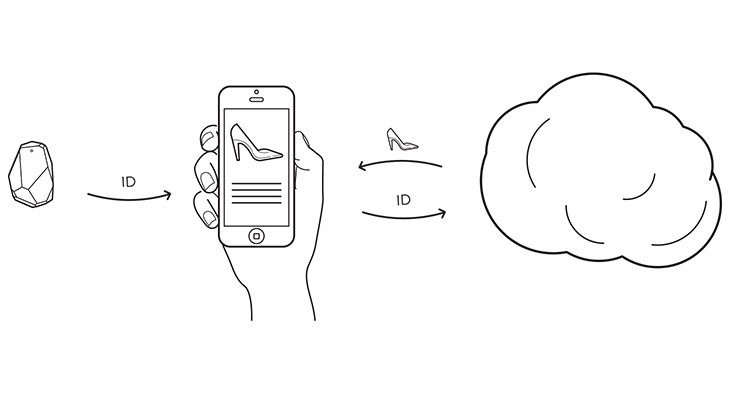
\includegraphics[width=8cm]{figuras/figura-2}}
 	}{
 	\Fonte{Estimote}			
 }	
\end{figure}
 
 \indent Segundo \cite{AppleInsider} iBeacons estão presentes em todas as lojas oficiais da Apple nos Estados Unidos. Através da utilização da aplicação oficial da loja e os iBeacons, os clientes podem ter acesso a uma camada extra de informações e serviços disponíveis nas lojas.
 
 \subsection{Eddystone}
 \label{sec:eddystone}
 
 Eddystone é um formato de beacon aberto do Google e que funciona com os sistemas Android e iOS. Eddystone inclui três tipos de estrutura para transmissão de dados, adequados para diferentes cenários. \cite{Google} \\
 \indent O padrão Eddystone é uma parte integrante da plataforma de beacons da Google. Com sua utilização é possível:
 
 \begin{itemize}
 	\item Permitir que as aplicações reajam ao contexto do usuário através de anexos (attachments) beacons;
 	\item Monitorar o status de uma frota de beacons a estrutura de telemetria do padrão Eddystone;
 	\item Transmitir dados para utilização da Web Física.
 \end{itemize}
 
 \begin{figure}[h!]
 	\centering
 	\Caption{\label{fig:exemplo-3} Dinâmica do padrão Eddystone}	
 	\UECEfig{}{
 		\fbox{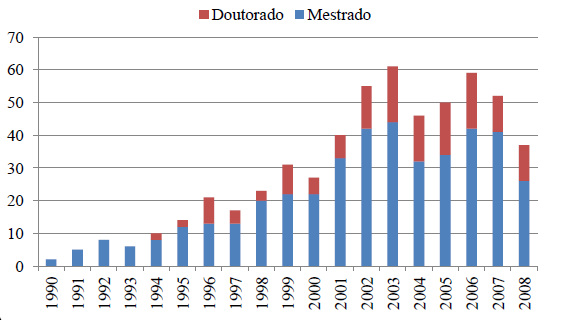
\includegraphics[width=8cm]{figuras/figura-3}}
 	}{
 	\Fonte{Google Developers}			
 }	
\end{figure}

A plataforma de beacons do Google é composta pelos próprios beacons, pelo padrão Eddystone e pela API de proximidade de beacons. \\
\indent Os beacons que suportam as especificações do padrão Eddystone podem transmitir dados de um único tipo de estrutura ou intercalar entre uma estrutura e outra. Por exemplo, transmitir repetidamente 50 estruturas do tipo Eddystone-UID seguidas de uma estrutura Eddystone-TLM. \\
\indent O padrão Eddystone especifica atualmente três tipos de estruturas: Eddystone-UID, Eddystone-URL e Eddystone-TLM.

\subsubsection{Eddystone-UID}
\label{sec:eddystone-uid}

Eddystone-UID contém o número identificador do beacon, que pode ser utilizado por um aplicação para disparar uma ação para o usuário. No Eddystone-UID, assim como ocorre no iBeacon, também é enviado um pequeno pacote de dados contendo um namespace e instance, detalhes no quadro abaixo:

\begin{quadro}[h!]	
	\centering
	\Caption{\label{qua:eddystone-UID} Informações presentes em um pacote de sinal em Eddystone}		
	\UECEqua{}{
		\begin{tabular}{|c|c|l|}
			\hline
			Campo & Tamanho & Descrição \\
			\hline
			Namespace & 10 bytes & Identificador de um conjunto de beacons\\
			\hline
			Instance & 6 bytes & Usado para identificar individualmente um beacon\\
			\hline
		\end{tabular}
	}{
	\Fonte{Elaborado pelo autor}
}
\end{quadro}

Para gerar um namespace a especificação do padrão Eddystone recomenda utilizar os dez primeiros bytes do hash SHA-1 gerado a partir de um nome de domínio. Exemplo de namespace gerado a partir do domínio ``fucapi.br'' utilizando a linguagem python:

\begin{figure}[h!]
	\centering
	\Caption{\label{fig:codigo-3} Código de exemplo para geração de namespace em python}	
	\UECEfig{}{
		\fbox{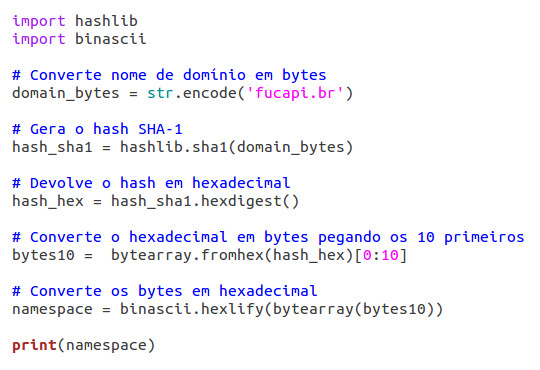
\includegraphics[width=8cm]{figuras/namespace_python}}
	}{
	\Fonte{Elaborado pelo autor}			
}	
\end{figure}

Ao executar o código a saída é:\\
\indent 1755ba6780003245d85c

\subsubsection{Eddystone-URL}
\label{sec:eddystone-url}

Eddystone-URL é a base para um novo conceito criado pela Google, chamado de Web Física, onde o usuário não precisará de um aplicativo dedicado para interpretar e executar as ações ao utilizar beacons fixados em objetos do mundo real. O conteúdo transmitido pelos beacons segue o mesmo padrão das URLs interpretadas pelos navegadores web, assim o usuário poderá acessar o conteúdo -- em forma de webapp ou website -- sem precisar baixar e instalar um aplicativo dedicado.

\subsubsection{Eddystone-TLM}
\label{sec:eddystone-tlm}

Eddystone-TLM especifica uma estrutura apropriada para transmissão de dados sobre os próprios beacons, permitindo que os mesmos possam ser gerenciados. Essa estrutura pode ser enviada juntamente com Eddystone-UID ou Eddystone-URL. A aplicação utilizada pelo usuário deve ser preparada para retransmitir os dados enviados pelo Eddystone-TLM para um serviço externo responsável por prover dados de gerenciamento. \\
\indent A estrutura pode conter os seguintes dados sobre os beacons:      

\begin{itemize}
	\item Tensão da bateria, que pode ser usado para estimar o nível de bateria restante em um beacon;
	\item Temperatura do beacon;
	\item Número de pacotes enviados desde a última vez que o beacon foi ligado ou reiniciado;
	\item Tempo de atividade desde a última vez que o beacon foi ligado ou reiniciado.
\end{itemize}
	%\chapter{Trabalhos Relacionados}
\label{cap:trabalhos-relacionados}

Integer non lacinia magna. Aenean tempor lorem tellus, non sodales nisl commodo ut. Proin mattis placerat risus sit amet laoreet. Praesent sapien arcu, maximus ac fringilla efficitur, vulputate faucibus sem. Donec aliquet velit eros, sit amet elementum dolor pharetra eget. Integer eget mattis libero

\section{Trabalho Relacionado A}
\label{sec:trabalho-relacionado-a}

\lipsum[10]

	\begin{figure}[h!]
		\centering
		\Caption{\label{fig:exemplo-1} Lorem ipsum dolor sit amet, consectetur adipiscing elit. Suspendisse commodo lectus et augue elementum varius.}	
		\UECEfig{}{
			\fbox{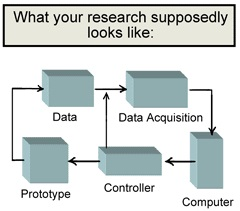
\includegraphics[width=8cm]{figuras/figura-1}}
		}{
			\Fonte{Elaborado pelo autor}
		}	
	\end{figure}
	
\lipsum[11]

\section{Trabalho Relacionado B}
\label{sec:trabalho-relacionado-b}

Integer non lacinia magna. Aenean tempor lorem tellus, non sodales nisl commodo ut. Proin mattis placerat risus sit amet laoreet. Praesent sapien arcu, maximus ac fringilla efficitur, vulputate faucibus sem. Donec aliquet velit eros, sit amet elementum dolor pharetra eget. Integer eget mattis libero. Praesent ex velit, pulvinar at massa vel, fermentum dictum mauris. Ut feugiat accumsan augue, et ultrices ipsum euismod vitae

	\begin{figure}[h!]
		\centering
		\Caption{\label{fig:exemplo-2} Maecenas luctus augue odio, sed tincidunt nunc posuere nec}	
		\UECEfig{}{
			\fbox{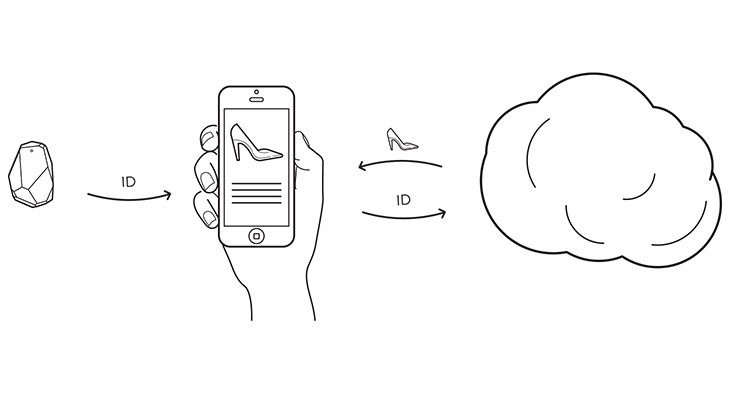
\includegraphics[width=8cm]{figuras/figura-2}}
		}{
			\Fonte{Elaborado pelo autor}			
		}	
	\end{figure}

Nunc ac pretium dui. Mauris aliquam dapibus nulla ac mattis. Aenean non tortor volutpat, varius lectus vitae, accumsan nibh. Cras pretium vestibulum enim, id ullamcorper tortor ultrices non. Integer sodales viverra faucibus. Curabitur at dui lacinia, rhoncus lacus at, blandit metus. Integer scelerisque non enim quis ornare.

	\begin{quadro}[h!]	
		\centering
		\Caption{\label{qua:exemplo-1} Praesent ex velit, pulvinar at massa vel, fermentum dictum mauris. Ut feugiat accumsan augue}		
		\UECEqua{}{
			\begin{tabular}{|c|c|l|l|}
				\hline
				Quisque & pharetra & tempus & vulputate \\
				\hline
				E1 & Complete coverage by a single transcript & Both  & Complete\\
				\hline
				E2 & Complete coverage by more than & Both splice sites & Complete\\
				\hline
				E3 & Partial coverage & Both splice sites & Both \\				
				\hline
			\end{tabular}
		}{
			\Fonte{Elaborado pelo autor}
		}
	\end{quadro}
	
\lipsum[20]

	
	\begin{quadro}[h!]	
		\centering
		\Caption{\label{qua:exemplo-2} Duis faucibus, enim quis tincidunt pellentesque}		
		\UECEqua{}{
			\begin{tabular}{|c|c|}
				\hline
				Quisque & pharetra \\
				\hline
				E1 & Complete coverage by a single transcript \\
				\hline
				E2 & Complete coverage by more than \\
				\hline
				E3 & Partial coverage \\
				\hline
				E4 & Partial coverage \\
				\hline
				E5 & Partial coverage \\
				\hline
				E6 & Partial coverage \\
				\hline
				E7 & Partial coverage \\
				\hline
			\end{tabular}
		}{
			\Fonte{Elaborado pelo autor}
		}
	\end{quadro}

\lipsum[21]

Integer non lacinia magna. Aenean tempor lorem tellus, non sodales nisl commodo ut. Proin mattis placerat risus sit amet laoreet. Praesent sapien arcu, maximus ac fringilla efficitur, vulputate faucibus sem. Donec aliquet velit eros, sit amet elementum dolor pharetra eget. Integer eget mattis libero.
\Gls{ambiguidade}
\Gls{braile}
\Gls{coerencia}
\Gls{dialetos}
\Gls{elipse}
\Gls{locucao-adjetiva}
\Gls{modificadores}
\Gls{paronimos}
\Gls{sintese}
\Gls{borboleta}
	%\chapter{Metodologia}
\label{chap:metodologia}

\lipsum[2]
\lipsum[12]

O autor \cite{lamport1986latex} e \cite{Maia2011} \lipsum[2] 

\begin{table}[h!]
	\Caption{\label{tabela-ibge} Um Exemplo de tabela alinhada que pode ser longa ou curta, conforme padrão IBGE. conforme padrão IBGE. conforme padrão IBGE. conforme padrão IBGE. conforme padrão IBGE. conforme padrão IBGE. conforme padrão IBGE. conforme padrão IBGE. conforme padrão IBGE. conforme padrão IBGE. conforme padrão IBGE.}%
	\IBGEtab{}{%
		\begin{tabular}{ccc}
			\toprule
			Nome & Nascimento & Documento \\
			\midrule \midrule
			Maria da Silva & 11/11/1111 & 111.111.111-11 \\
			Maria da Silva & 11/11/1111 & 111.111.111-11 \\
			Maria da Silva & 11/11/1111 & 111.111.111-11 \\
			\bottomrule
		\end{tabular}%
	}{%
	\Fonte{Produzido pelos autores}%
	\Nota{Esta éuma nota, que diz que os dados são baseados na
		regressão linear.}%
	\Nota[Anotações]{Uma anotação adicional, seguida de várias outras.}%
}
\end{table}

\cite{Huetal2000} \lipsum[2] 

\section{Exemplo de Algoritmos e Figuras}
\label{sec:exemplo-de-algoritmos-e-figuras}

\lipsum[2]

\begin{algorithm}[h!]
	\SetSpacedAlgorithm
	\caption{\label{exemplo-de-algoritmo}Como escrever algoritmos no \LaTeX2e}
	\Entrada{o proprio texto}
	\Saida{como escrever algoritmos com \LaTeX2e }
	\Inicio{
		inicializa\c{c}\~ao\;
		\Repita{fim do texto}{
			leia o atual\;
			\Se{entendeu}{
				vá para o próximo\;
				próximo se torna o atual\;}
			\Senao{volte ao início da seção\;}
		}
	}	
\end{algorithm}

\lipsum[2]
%\begin{algorithm}[H]
%	\Entrada{o proprio texto}
%	\Saida{como escrever algoritmos com \LaTeX2e }
%	\Inicio{
%		inicializa\c{c}\~ao\;
%		\Repita{fim do texto}{
%			leia o atual\;
%			\Se{entendeu}{
%				vá para o próximo\;
%				próximo se torna o atual\;}
%			\Senao{volte ao início da seção\;}
%		}
%	}
%	\caption{Exemplo de Algoritmo Versao 02}
%\end{algorithm}

%\begin{algorithm}
%	\begin{algorithmic}
%	\Entrada{o proprio texto}
%	\Saida{como escrever algoritmos com \LaTeX2e }	
%	\end{algorithmic}
%\end{algorithm}

Exemplo de alíneas com números:

\begin{alineascomnumero}
	\item Lorem ipsum dolor sit amet, consectetur adipiscing elit. Nunc dictum sed tortor nec viverra.
	\item Praesent vitae nulla varius, pulvinar quam at, dapibus nisi. Aenean in commodo tellus. Mauris molestie est sed justo malesuada, quis feugiat tellus venenatis.
	\item Praesent quis erat eleifend, lacinia turpis in, tristique tellus. Nunc dictum sed tortor nec viverra.
	\item Mauris facilisis odio eu ornare tempor. Nunc dictum sed tortor nec viverra.
	\item Curabitur convallis odio at eros consequat pretium.
\end{alineascomnumero}

\lipsum[12]

\begin{table}[h!]	
	\centering
	\Caption{\label{tab:internal}Internal exon scores}	
	\IBGEtab{}{
		\begin{tabular}{cll}
			\toprule
			Ranking & Exon Coverage & Splice Site Support\\
			\midrule \midrule
			E1 & Complete coverage by a single transcript & Both splice sites\\
			E2 & Complete coverage by more than a single transcript & Both splice sites\\
			E3 & Partial coverage & Both splice sites\\
			E4 & Partial coverage & One splice site\\
			E5 & Complete or partial coverage & No splice sites\\
			E6 & No coverage & No splice sites\\
			\bottomrule
		\end{tabular}
	}{
	\Fonte{os autores}
}
\end{table}

\lipsum[2] Referenciando a \autoref{tab:internal} \lipsum[2]

\index{figuras}Figuras podem ser criadas diretamente em LaTeX,
como o exemplo da \ref{fig-grafico-1}.

\begin{figure}[h!]
	\centering
	\Caption{\label{fig-grafico-1}Produção anual das dissertações de mestrado e teses de doutorado entre os anos de 1990 e 2008}		
	\IBGEtab{}{
		\fbox{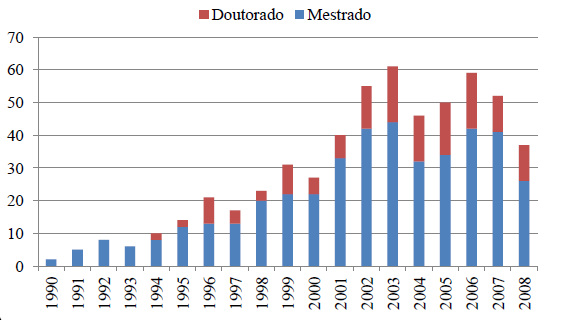
\includegraphics[scale=0.5]{figuras/figura-3}}
	}{
	\Fonte{os autores}
}
\end{figure}

Ou então figuras podem ser incorporadas de arquivos externos, como é o caso da \autoref{fig-grafico-1}. Se a figura que ser incluída se tratar de um diagrama, um gráfico ou uma ilustração que você mesmo produza, priorize o uso de imagens vetoriais no formato PDF. Com isso, o tamanho do arquivo final do trabalho será menor, e as imagens terão uma apresentação melhor, principalmente quando impressas, uma vez que imagens vetorias são perfeitamente escaláveis para qualquer dimensão. Nesse caso, se for utilizar o Microsoft Excel para produzir gráficos, ou o Microsoft Word para produzir ilustrações, exporte-os como PDF e os incorpore ao documento conforme o exemplo abaixo. No entanto, para manter a coerência no uso de software livre (já que você está usando LaTeX e abnTeX),  teste a ferramenta InkScape\index{InkScape}. ao CorelDraw\index{CorelDraw} ou ao Adobe Illustrator\index{Adobe! Illustrator}.  De todo modo, caso não seja possível  utilizar arquivos de imagens como PDF, utilize qualquer outro formato, como JPEG, GIF, BMP, etc.  Nesse caso, você pode tentar aprimorar as imagens incorporadas com o software livre \index{Gimp}Gimp. Ele é uma alternativa livre ao Adobe Photoshop\index{Adobe! Photoshop}.

\section{Usando Fórmulas Matemáticas}

\lipsum[2]

	\begin{equation}
		\begin{aligned}
			x = a_0 + \cfrac{1}{a_1
				+ \cfrac{1}{a_2
					+ \cfrac{1}{a_3 + \cfrac{1}{a_4} } } }
		\end{aligned}
	\end{equation}

\lipsum[3]

	\begin{equation}
		\begin{aligned}
			k_{n+1} = n^2 + k_n^2 - k_{n-1}
		\end{aligned}
	\end{equation}

\lipsum[4]

	\begin{equation}
		\begin{aligned}
			\cos (2\theta) = \cos^2 \theta - \sin^2 \theta
		\end{aligned}
	\end{equation}
	
\lipsum[5]

	\begin{equation}
		\begin{aligned}
			A_{m,n} =
			\begin{pmatrix}
			a_{1,1} & a_{1,2} & \cdots & a_{1,n} \\
			a_{2,1} & a_{2,2} & \cdots & a_{2,n} \\
			\vdots  & \vdots  & \ddots & \vdots  \\
			a_{m,1} & a_{m,2} & \cdots & a_{m,n}
			\end{pmatrix}
		\end{aligned}
	\end{equation}

\lipsum[6]

	\begin{equation}
		\begin{aligned}
			f(n) = \left\{ 
			\begin{array}{l l}
			n/2 & \quad \text{if $n$ is even}\\
			-(n+1)/2 & \quad \text{if $n$ is odd}
			\end{array} \right.
		\end{aligned}
	\end{equation}
	
\lipsum[7]

\section{Usando Algoritmos}

\lipsum[8]

\begin{algorithm}[h!]
	\SetSpacedAlgorithm
	\caption{\label{alg:algoritmo_de_colonica_de_formigas}Algoritmo de Otimização por Colônia de Formiga}
	\Entrada{Entrada do Algoritmo}
	\Saida{Saida do Algoritmo}
	\Inicio{
		Atribua os valores dos parâmetros\;
		Inicialize as trilhas de feromônios\;
		\Enqto{não atingir o critério de parada}{
			\Para{cada formiga}{
				Construa as Soluções\;
			}
			Aplique Busca Local (Opcional)\;
			Atualize o Feromônio\;
		}	
	}		
\end{algorithm}

\lipsum[9]

\section{Usando Código-fonte}

\lipsum[10]

\lstinputlisting[language=C++,caption={Hello World em C++}]{figuras/main.cpp}

\lipsum[11]

\begin{lstlisting}[language=Java,caption={Hello World em Java}]
public class HelloWorld {
	public static void main(String[] args) {
		System.out.println("Hello World!");
	}
}
\end{lstlisting}

\lipsum[11]

\section{Usando Teoremas, Proposições, etc}

Lorem ipsum dolor sit amet, consectetur adipiscing elit. Nunc dictum sed tortor nec viverra. consectetur adipiscing elit. Nunc dictum sed tortor nec viverra.

\begin{teo}[Pitágoras]
	Em todo triângulo retângulo o quadrado do comprimento da
	hipotenusa é igual a soma dos quadrados dos comprimentos dos catetos.
\end{teo}


Lorem ipsum dolor sit amet, consectetur adipiscing elit. Nunc dictum sed tortor nec viverra. consectetur adipiscing elit. Nunc dictum sed tortor nec viverra.

\begin{teo}[Fermat]
	Não existem inteiros $n > 2$, e $x, y, z$ tais que $x^n + y^n = z$
\end{teo}

Lorem ipsum dolor sit amet, consectetur adipiscing elit. Nunc dictum sed tortor nec viverra. consectetur adipiscing elit. Nunc dictum sed tortor nec viverra.

\begin{prop}
	Para demonstrar o Teorema de Pitágoras...
\end{prop}

Lorem ipsum dolor sit amet, consectetur adipiscing elit. Nunc dictum sed tortor nec viverra. consectetur adipiscing elit. Nunc dictum sed tortor nec viverra.

\begin{exem}
	Este é um exemplo do uso do ambiente exe definido acima.
\end{exem}

Lorem ipsum dolor sit amet, consectetur adipiscing elit. Nunc dictum sed tortor nec viverra. consectetur adipiscing elit. Nunc dictum sed tortor nec viverra.

\begin{xdefinicao}
	Definimos o produto de ...
\end{xdefinicao}

Lorem ipsum dolor sit amet, consectetur adipiscing elit. Nunc dictum sed tortor nec viverra. consectetur adipiscing elit. Nunc dictum sed tortor nec viverra.

\section{Usando Questões}


Lorem ipsum dolor sit amet, consectetur adipiscing elit. Nunc dictum sed tortor nec viverra. consectetur adipiscing elit. Nunc dictum sed tortor nec viverra.

\begin{questao}
	\item Esta é a primeira questão com alguns itens:
		\begin{enumerate}
			\item Este é o primeiro item
			\item Segundo item
		\end{enumerate}
	\item Esta é a segunda questão:
		\begin{enumerate}
			\item Este é o primeiro item
			\item Segundo item
		\end{enumerate}
	\item Lorem ipsum dolor sit amet, consectetur adipiscing elit. Nunc dictum sed tortor nec viverra. consectetur adipiscing elit. Nunc dictum sed tortor nec viverra.
		\begin{enumerate}
			\item consectetur
			\item adipiscing
			\item Nunc
			\item dictum
		\end{enumerate}
\end{questao}

\section{Citações}

\subsection{Documentos com três autores}

Quando houver três autores na citação, apresentam se os três, separados por ponto e vírgula, caso estes estejam após o texto. Se os autores estiverem incluídos no texto, devem ser separados por vírgula e pela conjunção "e".

\citeautoronline{tresautores}

\cite{tresautores}

\subsection{Documentos com mais de três autores}
Havendo mais de três autores, indica-se o primeiro seguido da expressão \textit{et al.} (do latim \textit{et alli}, que significa e outros), do ano e da página.

\citeautoronline{quatroautores}

\cite{quatroautores}

\subsection{Documentos de vários autores}

Havendo    citações    indiretas de    diversos    documentos    de    vários    autores, mencionados  simultaneamente e  que  expressam  a  mesma  ideia,  separam-se  os  autores  por ponto e vírgula, em ordem alfabética.

\cite{tresautores, quatroautores}

\section{Notas de Rodap\'{e}}

Deve-se utilizar o sistema autor-data para as  citações no texto e o numérico para notas explicativas\footnote{Veja - se como exemplo desse tipo de abordagem o estudo de Netzer (1976)}. As notas de rodapé podem e devem ser alinhadas, a partir da segunda linha da mesma nota, abaixo da primeira letra da primeira palavra, de forma a destacar o expoente \footnote{Encontramos  esse  tipo  de  perspectiva  na  2ª  parte  do  verbete  referido  na  nota  anterior,  em  grande  parte  do estudo de Rahner (1962).} e sem espaço entre elas e com fonte menor (tamanho 10).


	%\chapter{Resultados}
\label{chap:resultados}

\lipsum[2]

\section{Resultados do Experimento A}
\label{sec:resultados-do-experimento-a}

\lipsum[3]

\section{Resultados do Experimento B}
\label{sec:resultados-do-experimento-b}

\lipsum[4]
	%\chapter{Conclusões e Trabalhos Futuros}
\label{chap:conclusoes-e-trabalhos-futuros}

\lipsum[2]
\lipsum[34]

\section{Contribuições do Trabalho}
\label{sec:contribuicoes-do-trabalho}

\lipsum[3]

\section{Limitações}
\label{sec:limitacoes}

\lipsum[4]

\section{Trabalhos Futuros}
\label{sec:trabalhos-futuros}

\lipsum[5]





	
	%Elementos pós-textuais	
	%\bibliography{elementos-pos-textuais/referencias}
	%\imprimirglossario	
	%\imprimirapendices
		% Adicione aqui os apendices do seu trabalho
		%\apendice{Lorem Ipsum}
\label{ap:lorem-ipsum}

\lipsum[1]
		%\apendice{Modelo de Capa}
\label{ap:modelo-de-capa}

\lipsum[1]

		%\apendice{Termo de Fiel Depositário}
\label{ap:termo-de-fiel-depositario}

\noindent \textbf{Pesquisa:} ANÁLISE DA MORTALIDADE INFANTIL COM MALFORMAÇÕES CONGÊNITAS.

\noindent Pelo presente instrumento que atende às exigências legais, a Sra. Maria Consuelo Martins Saraiva, ``fiel depositário'' com o cargo de Secretária Municipal de Saúde de Iracema, após ter tomado conhecimento do protocolo de pesquisa intitulado: ANÁLISE DA MORTALIDADE INFANTIL COM MALFORMAÇÕES CONGÊNITAS. Analisando a repercussão desse estudo no contexto da saúde pública e epidemiologia, autoriza Karla Maria da Silva Lima, enfermeira, aluna do Curso de Mestrado Acadêmico em Enfermagem da Universidade Estadual do Ceará (UECE), sob orientação do Prof. Dr. José Maria de Castro, da UECE, ter acesso aos bancos de dados do Sistema de Informação sobre Nascidos Vivos e do Sistema de Informação sobre Mortalidade da Secretaria Municipal de Saúde de Iracema, objeto deste estudo, e que se encontram sob sua total responsabilidade. Fica claro que o Fiel Depositário pode a qualquer momento retirar sua AUTORIZAÇÃO e ciente de que todas as informações prestadas tornar-se-ão confidenciais e guardadas por força de sigilo profissional, assegurando que os dados obtidos da pesquisa serão somente utilizados para estudo.	
	%\imprimiranexos
		% Adicione aqui os anexos do seu trabalho
		%\anexo{Exemplo de Anexo}
\label{an:exemplo-de-anexo}

\lipsum[13]		
		%\anexo{Dinâmica das classes sociais}
\label{an:dinamica-das-classes-sociais}

\lipsum[14]
\index{AAA}
	%\imprimirindice

\end{document}